\documentclass[aspectratio=169]{beamer}
\usepackage{will_handley_beamer}
\usepackage{title_page}

% Commands
% --------
% - \arxiv{arxiv number}
% - \arxiv{<number>}            arxiv.org/abs/<number>
% - \oldarxiv{<arxiv number>}   arxiv.org/<number>
% - \doi{<doi>}                 doi.org/<doi>
% - \xkcd{<number>}             xkcd.com/<number>
% - \email{<email>}             <<email>>
% - \tthref{<website>}          <website>
% - \av[dist]{<quantity>}       <quantity>_{dist}
% - \student{<name>}{<detail>}{<photo>}

% Talk details
% ------------
\title{Next-Generation Model Comparison for Primordial Cosmology}
\date{LMU-Cambridge Partnership 2025}

\begin{document}

\begin{frame}
    \titlepage
\end{frame}

\begin{frame}
    \frametitle{Beginning the golden age of astronomy data}
    \begin{columns}
        \column{0.47\textwidth}
        \begin{itemize}
            \item Over our research lifetimes we will see next-generation data rates across the electromagnetic spectrum \& beyond:
                \begin{description}
                    \item[Radio] SKA \textit{et al}
                    \item[Micro] SO/CMB-S4/LiteBIRD
                    \item[IR] JWST, Roman
                    \item[Optical] Euclid, DESI, Rubin, EELT
                    \item[X-ray] Athena
                    \item[Gamma-ray] e-ASTROGAM
                    \item[Gravitational] LIGO/LVK$^+$/LISA
                    \item[Particle] CTA, IceCube, KM3NeT
                \end{description}
        \end{itemize}
        \column{0.55\textwidth}

        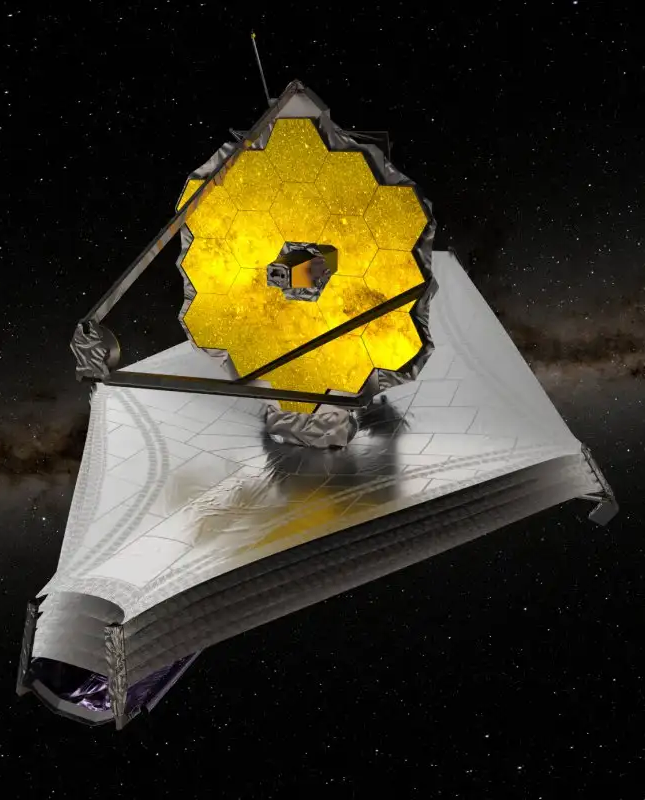
\includegraphics[height=0.145\textwidth]{figures/telescopes/jwst.png}%
        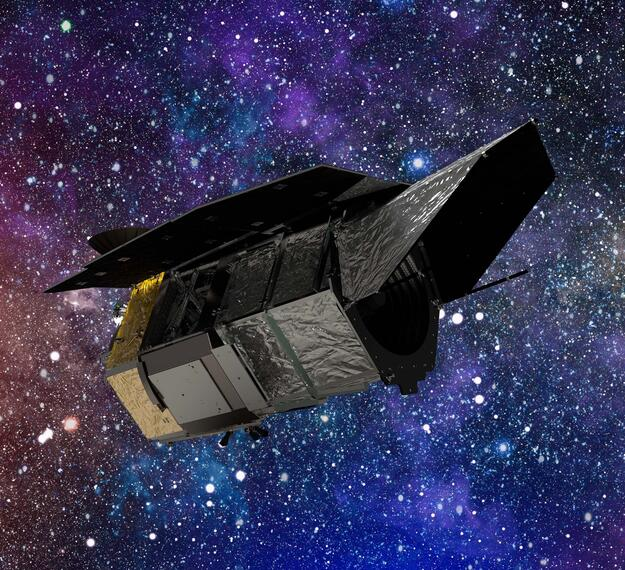
\includegraphics[height=0.145\textwidth]{figures/telescopes/roman.jpg}%
        \includegraphics[height=0.145\textwidth]{figures/telescopes/euclid.jpeg}%
        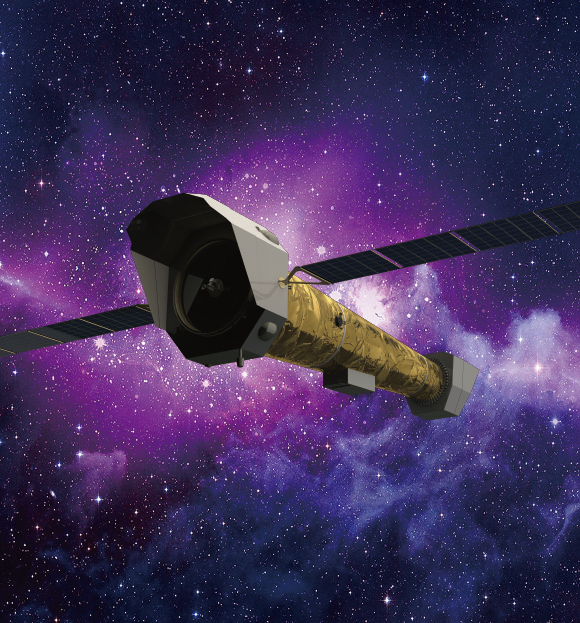
\includegraphics[height=0.145\textwidth]{figures/telescopes/athena.jpg}%
        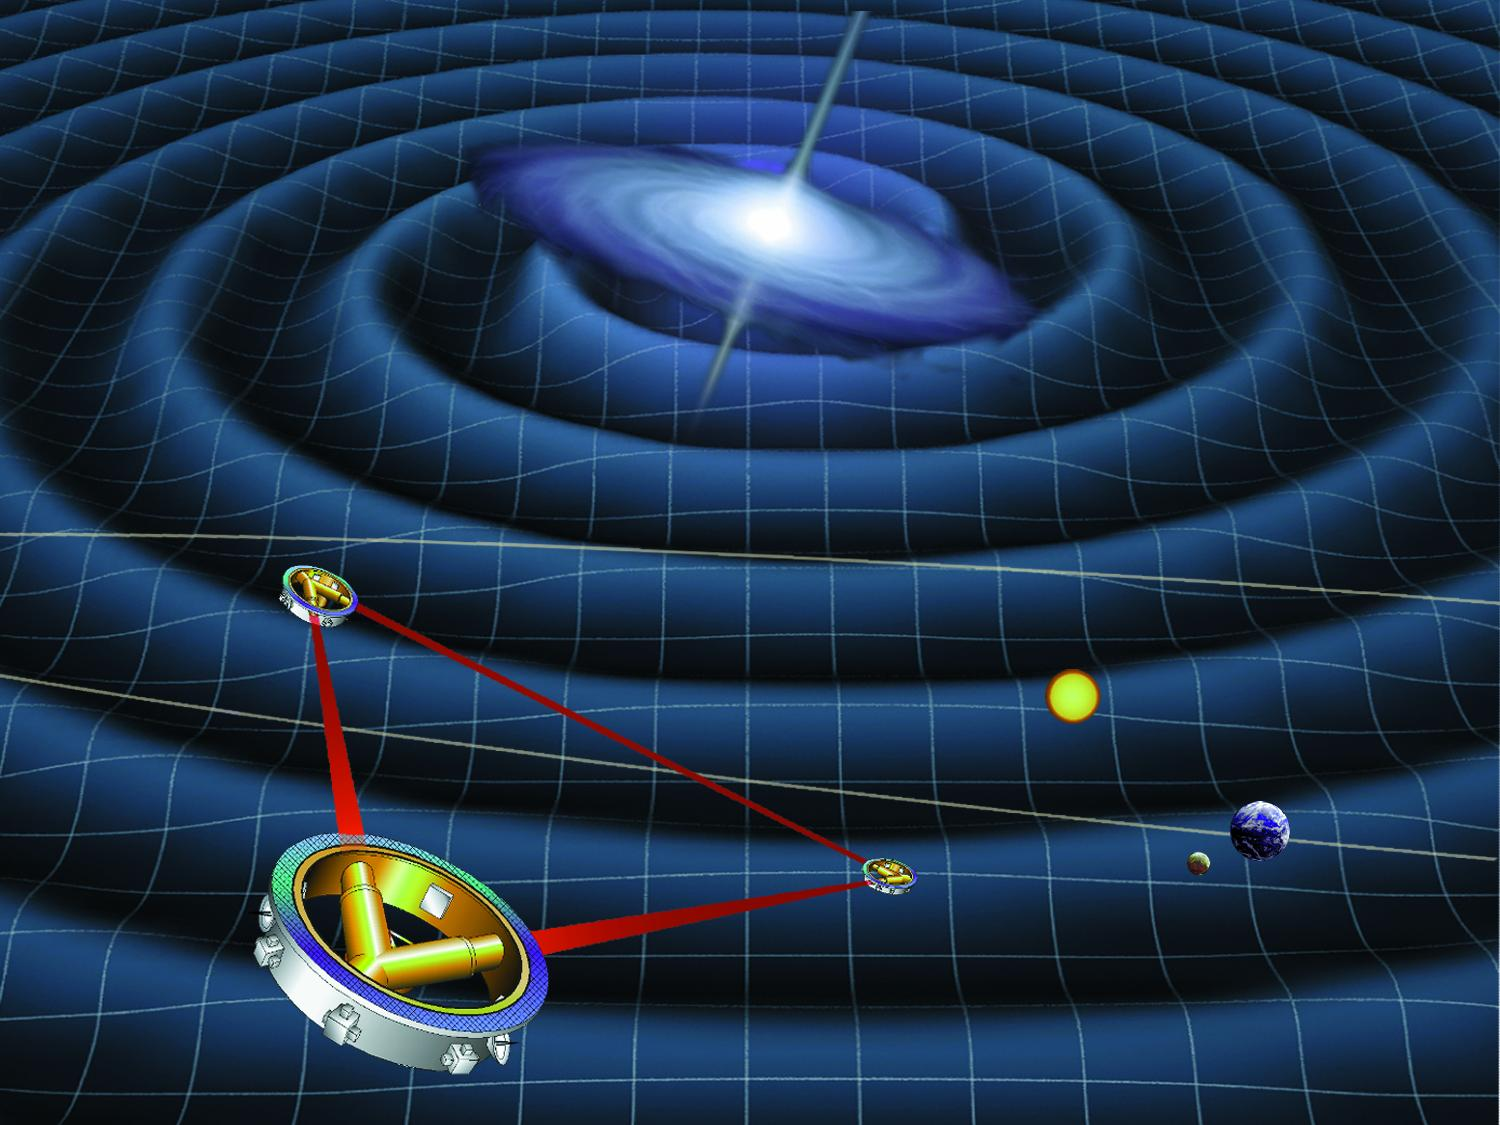
\includegraphics[height=0.145\textwidth]{figures/telescopes/lisa.jpg}%
        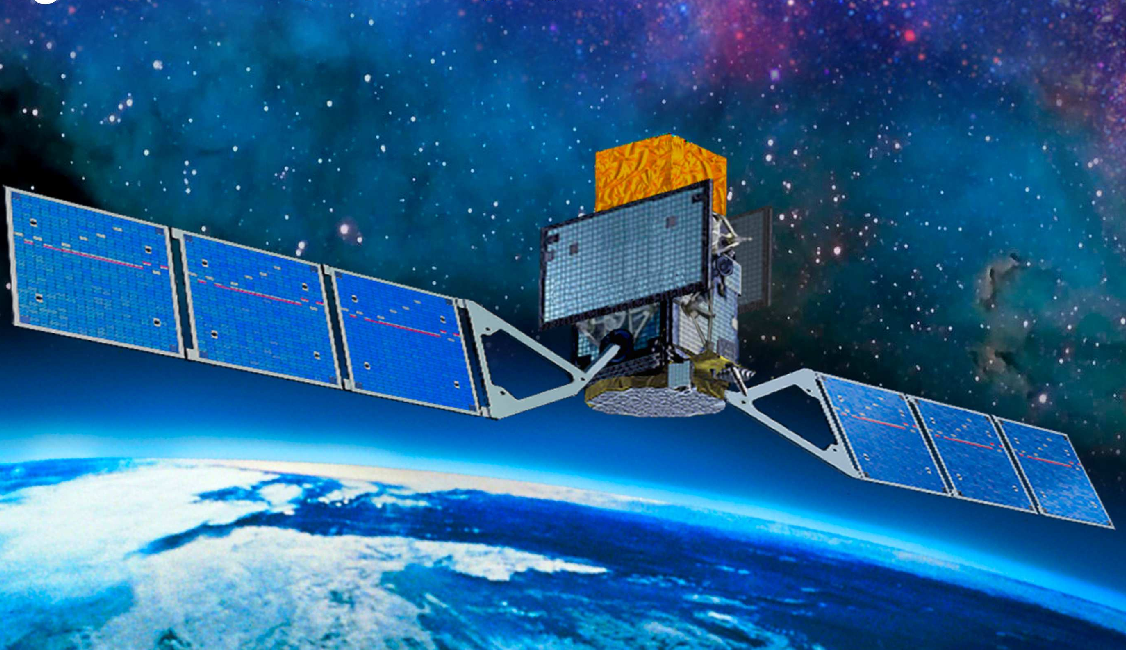
\includegraphics[height=0.145\textwidth]{figures/telescopes/e-ASTROGAM.pdf}%
        \vspace{-1pt}

        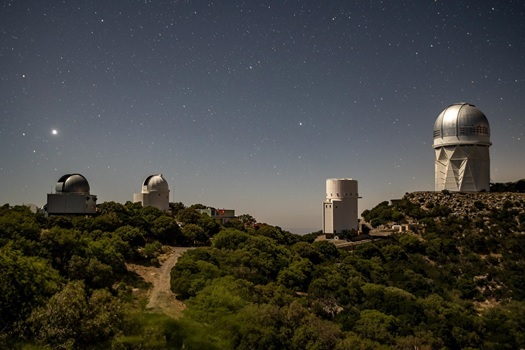
\includegraphics[height=0.15183\textwidth]{figures/telescopes/desi.jpg}%
        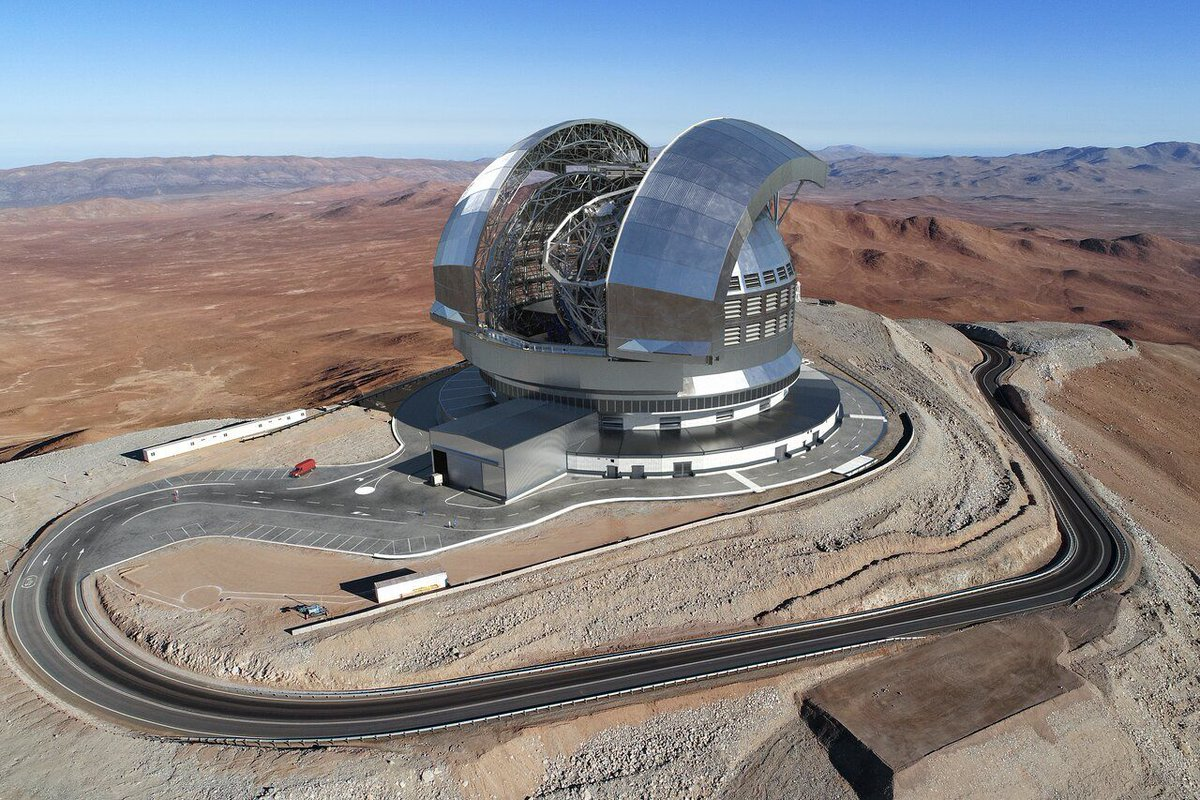
\includegraphics[height=0.15183\textwidth]{figures/telescopes/eelt.jpg}%
        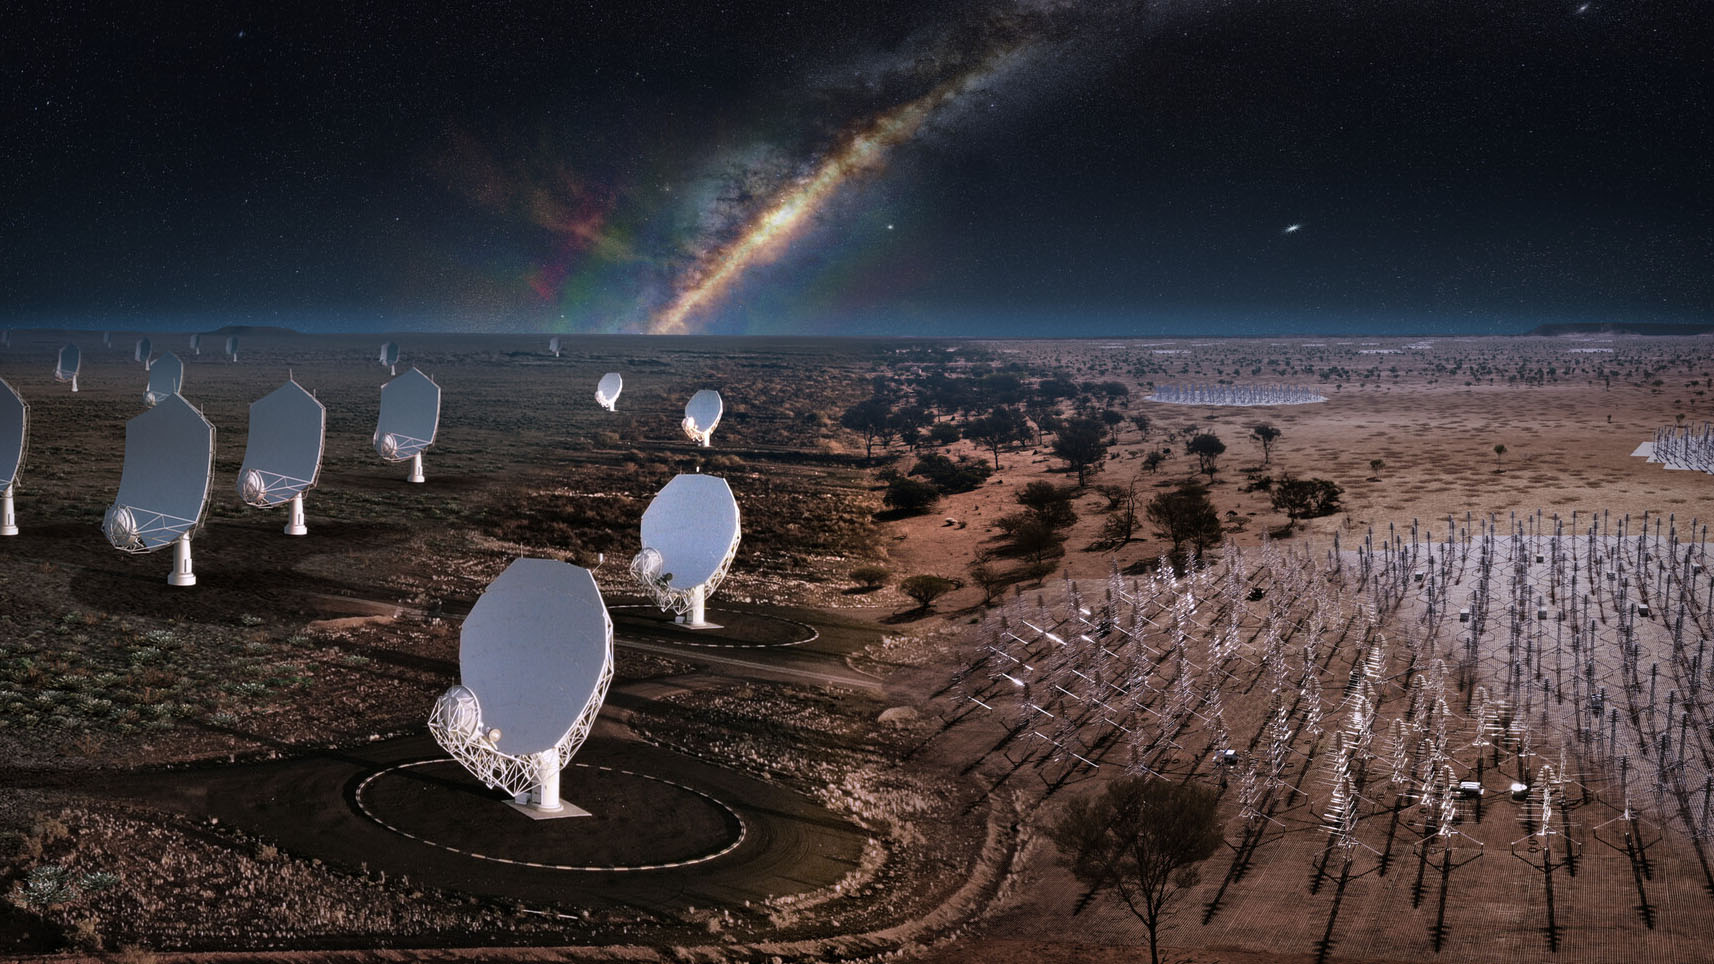
\includegraphics[height=0.15183\textwidth]{figures/telescopes/ska.jpg}%
        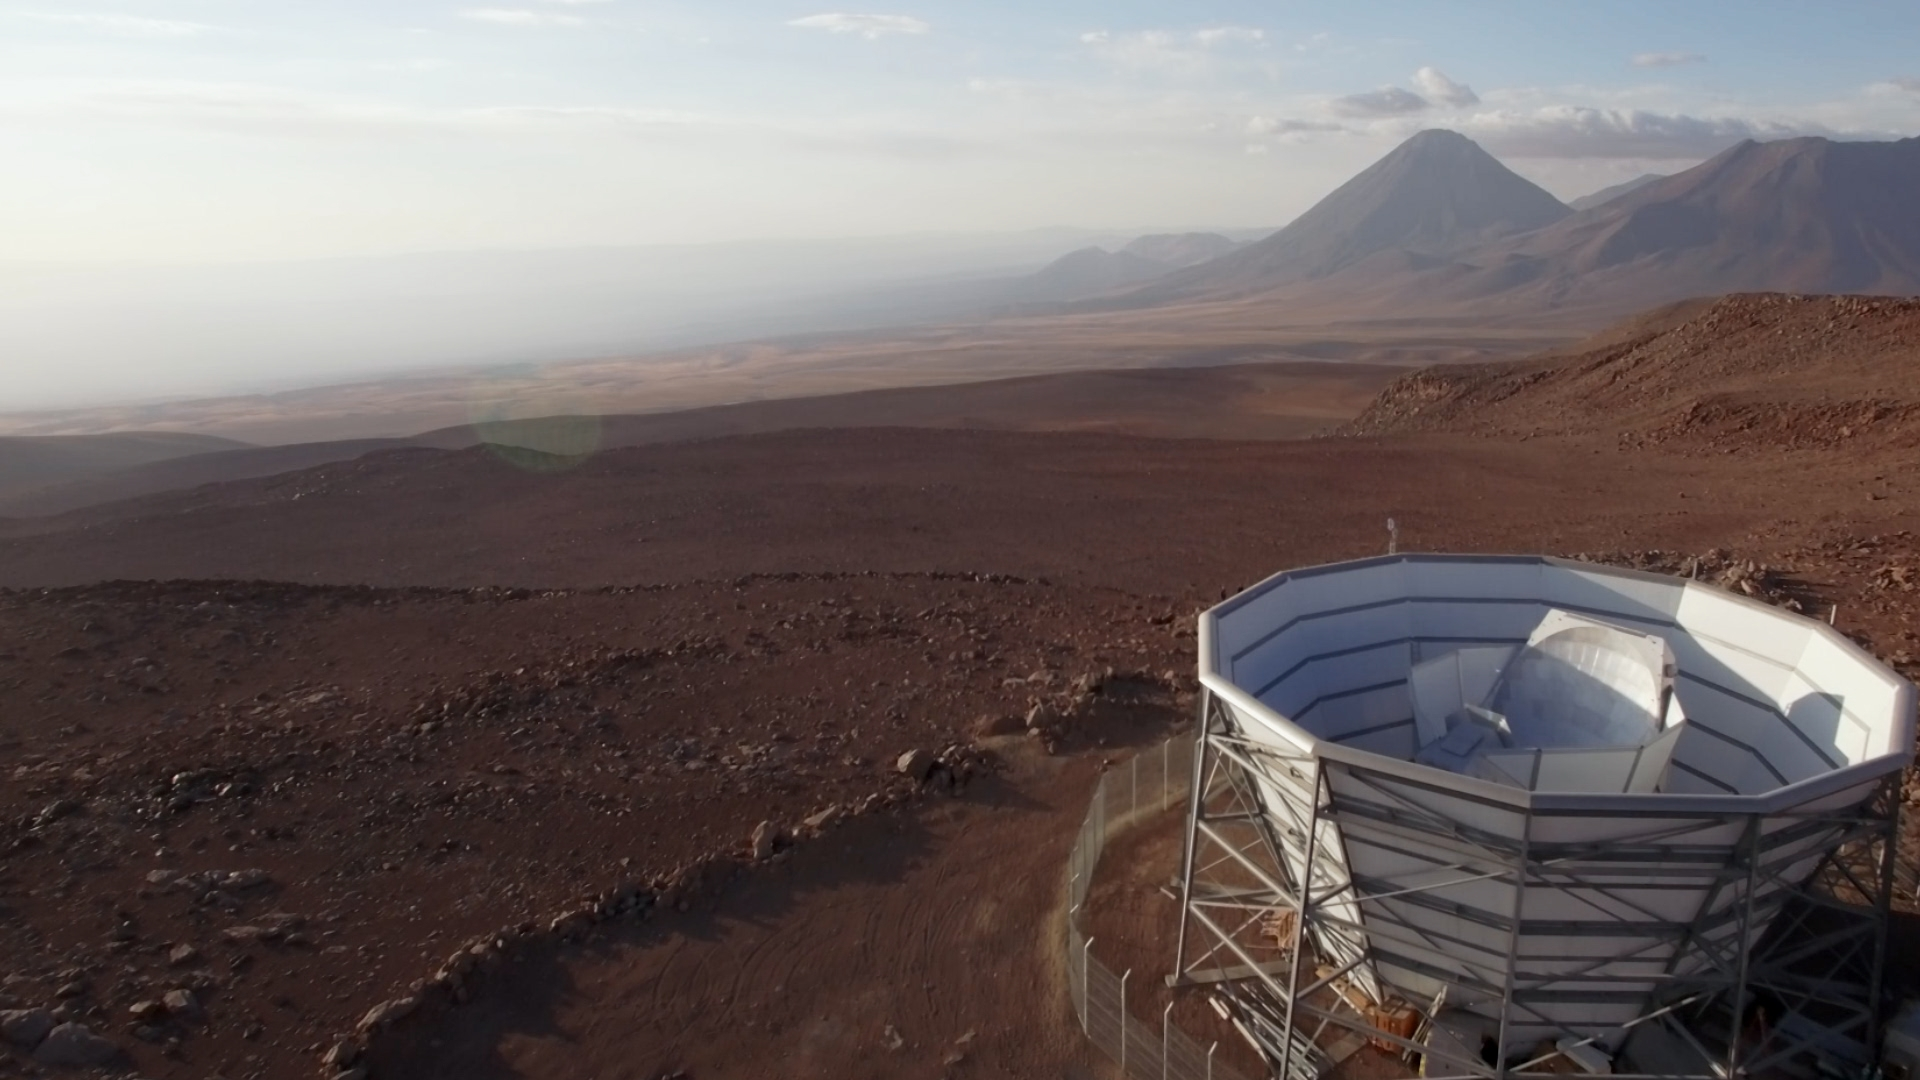
\includegraphics[height=0.15183\textwidth]{figures/telescopes/SO.jpg}%
        \vspace{-1pt}

        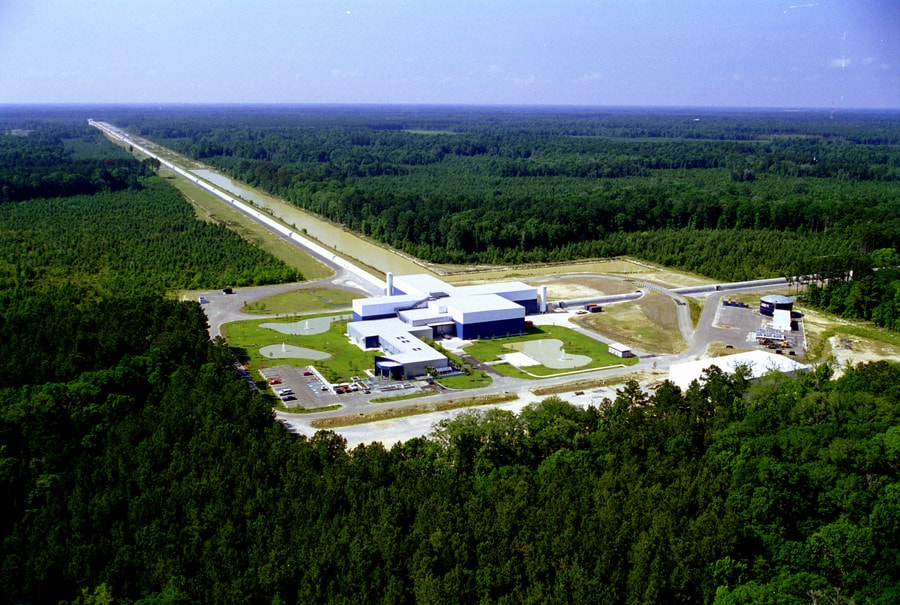
\includegraphics[height=0.18428\textwidth]{figures/telescopes/ligo.jpg}%
        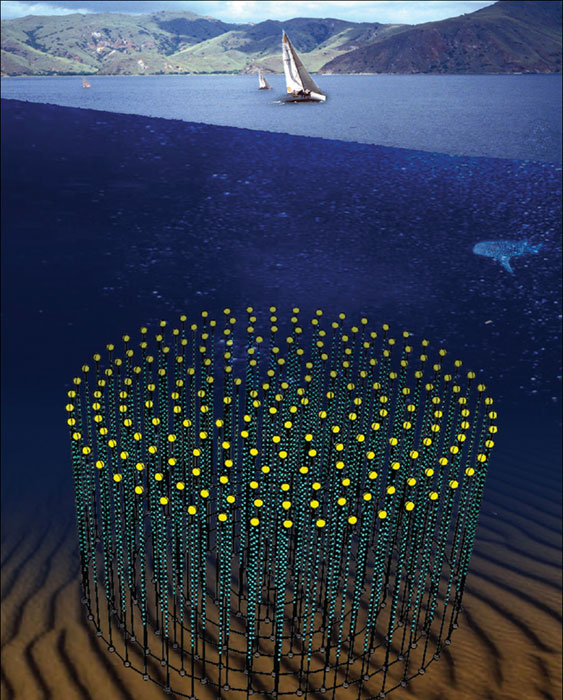
\includegraphics[height=0.18428\textwidth]{figures/telescopes/km3n.jpg}%
        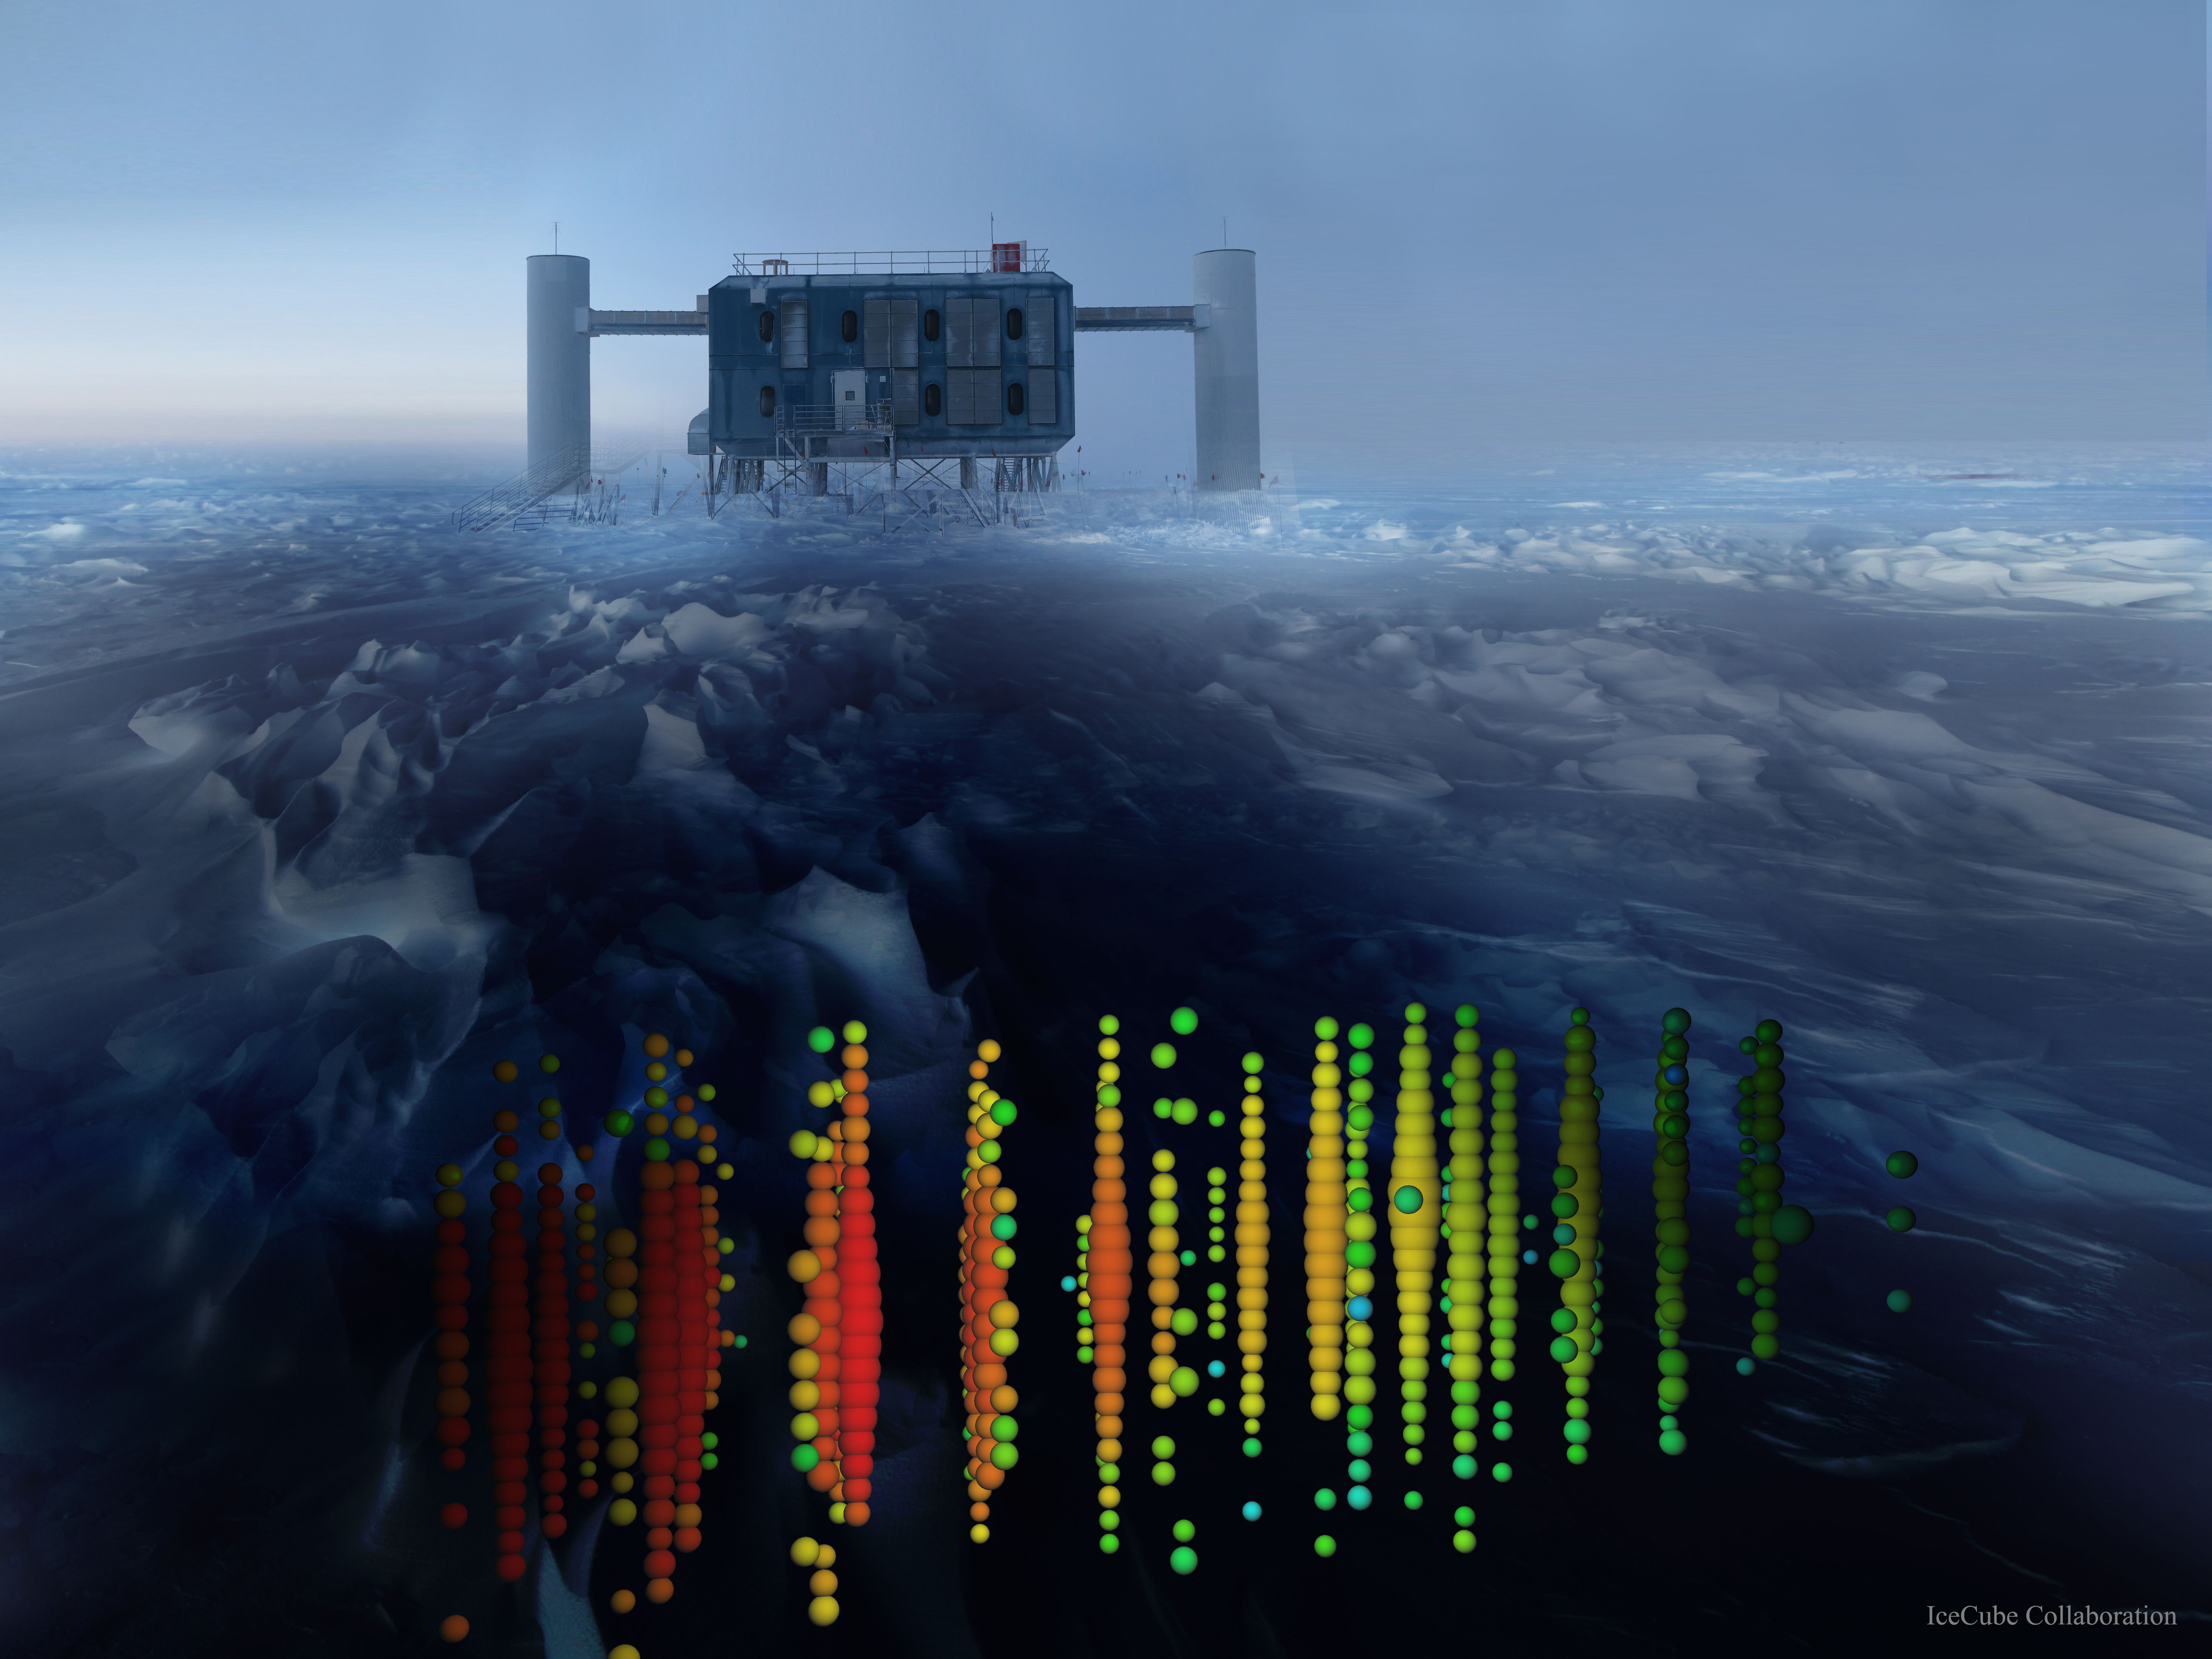
\includegraphics[height=0.18428\textwidth]{figures/telescopes/icecube.jpg}%
        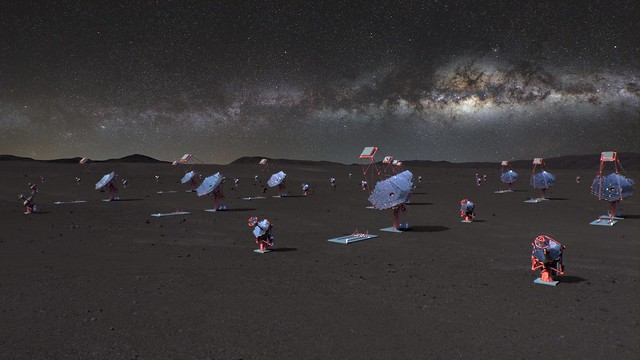
\includegraphics[height=0.18428\textwidth]{figures/telescopes/CTA.jpg}%

        \begin{itemize}
            \item This data deluge creates unprecedented computational challenges for model comparison and parameter estimation.
            \item Traditional computing approaches will not scale to these next-generation data volumes and complexity.
        \end{itemize}

    \end{columns}
\end{frame}

\begin{frame}
    \frametitle{GPU Computing: Beyond Machine Learning}
    \begin{columns}
        \column{0.48\textwidth}
        \begin{block}{GPU vs CPU for Scientific Computing}
            \begin{itemize}
                \item \textbf{CPU}: Few powerful cores (10s), complex control
                \item \textbf{GPU}: Many simple cores (1000s), simple control
                \item \textbf{Memory bandwidth}: GPU ~10× faster than CPU
                \item \textbf{Perfect for}: Independent parallel tasks
                \item \textbf{Scientific algorithms}: MCMC chains, likelihood evaluations, simulations
            \end{itemize}
        \end{block}
        \column{0.48\textwidth}
        \begin{block}{HPC Landscape Evolution}
            \begin{itemize}
                \item HPC transitioning to GPU-based architectures
                \item ML adoption accelerating hardware development
                \item Legacy CPU codes require modernization
            \end{itemize}
        \end{block}
        \begin{block}{Key Point}
            \begin{center}
                \textbf{GPU $\neq$ Machine Learning}\\
                GPUs accelerate any parallel algorithm
            \end{center}
        \end{block}
    \end{columns}
\end{frame}

\begin{frame}
    \frametitle{Modern Languages: Two Independent Capabilities}
    \begin{columns}
        \column{0.48\textwidth}
        \begin{block}{Capability 1: Automatic Differentiation}
            \begin{itemize}
                \item \textbf{Gradients ``for free''}: $\nabla_\theta \log \mathcal{L}(\theta)$
                \item Enables gradient-based MCMC (HMC, NUTS)
                \item Forward-mode, reverse-mode AD
                \item Essential for modern optimization
                \item \textbf{Example}: $\mathcal{O}(1)$ gradient computation regardless of parameter dimensionality
            \end{itemize}
        \end{block}
        \begin{block}{Capability 2: Massive Parallelization}
            \begin{itemize}
                \item \textbf{Vectorization across ensembles}
                \item JAX: \texttt{vmap}, \texttt{pmap} primitives
                \item PyTorch: \texttt{torch.vmap}
                \item Julia: Native array broadcasting
                \item \textbf{Example}: 1000 parallel chains/particles
            \end{itemize}
        \end{block}
        \column{0.48\textwidth}
        \begin{block}{Key Insight: Often Confused!}
            \begin{center}
                \textbf{These are completely independent!}\\
                \vspace{5pt}
                \textbf{People mistake one for the other}\\
                \vspace{10pt}
                You can use gradients on CPU\\
                You can parallelize without gradients\\
                \vspace{5pt}
                \textbf{Usually you only need one}
            \end{center}
        \end{block}
        \begin{block}{Traditional Physics Benefits}
            \begin{itemize}
                \item \textbf{Nested sampling}: Massive parallelization
                \item \textbf{Boltzmann solvers}: Vectorized across $k$-modes
                \item \textbf{N-body sims}: GPU acceleration
                \item \textbf{No ML required}: Classical algorithms win
            \end{itemize}
        \end{block}
    \end{columns}
\end{frame}

\begin{frame}
    \frametitle{Classical Algorithms on GPU Beat the ML Gold Rush}
    \student{toby_lovick}{Toby Lovick}{PhD}
    \begin{columns}
        \column{0.55\textwidth}
        \begin{block}{CMB Power Spectrum (6 params)}
            \begin{itemize}
                \item \textbf{PolyChord (CPU)}: ~1 hour
                \item \textbf{BlackJAX (GPU)}: 12 seconds
            \end{itemize}
            \begin{center}
                \textbf{300× speedup}
            \end{center}
        \end{block}
        \begin{block}{Cosmic Shear (37 params)}
            \begin{itemize}
                \item \textbf{PolyChord (48 CPUs)}: ~8 months
                \item \textbf{NUTS (12 A100 GPUs)}: 2 days
                \item \textbf{BlackJAX (1 A100 GPU)}: 4.5 hours
            \end{itemize}
            \begin{center}
                \textbf{$>$1000× speedup vs CPU}\\
                \textbf{10× speedup vs existing GPU approach}\arxiv{2405.12965}
            \end{center}
        \end{block}
        \includegraphics<1>[width=\textwidth]{figures/wl_corner.pdf}%
        \includegraphics<2>[width=\textwidth]{figures/wl_scaling.pdf}
        \vspace{10pt}
        \begin{block}{Key Insight: Classical > ML Gold Rush}
            \begin{itemize}
                \item \textbf{No machine learning}: Pure nested sampling
                \item \textbf{Statistical guarantees}: Proper uncertainties + evidence
                \item \textbf{Factor in training costs}: ML often slower end-to-end
                \item \textbf{Transparent algorithms}: No black boxes
            \end{itemize}
        \end{block}
    \end{columns}
\end{frame}

\begin{frame}
    \frametitle{AI-Accelerated Development: The Only Way Forward}
    \begin{columns}
        \column{0.48\textwidth}
        \begin{block}{The GPU Porting Challenge}
            \begin{itemize}
                \item \textbf{Massive undertaking}: Legacy CPU $\rightarrow$ GPU-native
                \item \textbf{Algorithmic complexity}: Vectorization, memory management
                \item \textbf{Language barriers}: Fortran/C++ $\rightarrow$ JAX/PyTorch
                \item \textbf{Scale problem}: Decades of scientific code
            \end{itemize}
        \end{block}
        \begin{block}{AI as Development Accelerator}
            \begin{itemize}
                \item \textbf{Code generation}: Automated translation
                \item \textbf{Debugging assistance}: Error analysis and fixes
                \item \textbf{Optimization guidance}: Performance bottleneck identification
                \item \textbf{Documentation}: Auto-generated comments and docs
            \end{itemize}
        \end{block}
        \column{0.48\textwidth}
        \begin{block}{Our Group's Wholehearted Embrace}
            \begin{itemize}
                \item \textbf{AI-first development}: Every project uses LLM assistance
                \item \textbf{Code review loops}: AI + human verification
                \item \textbf{Rapid prototyping}: Ideas to GPU code in hours
                \item \textbf{Quality control}: Human oversight remains critical
            \end{itemize}
        \end{block}
        \begin{block}{The Productivity Reality}
            \begin{itemize}
                \item \textbf{10× development speedup}: Personal experience
                \item \textbf{Focus shift}: Writing code $\rightarrow$ algorithm design
                \item \textbf{Democratization}: GPU programming accessible to all
            \end{itemize}
        \end{block}
    \end{columns}
\end{frame}

\begin{frame}
    \frametitle{Cambridge-LMU Synergies: Enabling Cross-Correlation Science}
    \begin{columns}
        \column{0.48\textwidth}
        \begin{block}{Cambridge Strengths}
            \begin{itemize}
                \item \textbf{CMB expertise}: Planck, SO, CMB-S4
                \item \textbf{Nested sampling}: PolyChord, BlackJAX-NS
                \item \textbf{GPU infrastructure}: Wilkes-3, Dawn
                \item \textbf{Bayesian inference}: Model comparison, evidence
            \end{itemize}
        \end{block}
        \begin{block}{LMU Munich Strengths}
            \begin{itemize}
                \item \textbf{Galaxy surveys}: DESI, Euclid expertise
                \item \textbf{Large-scale structure}: N-body simulations
                \item \textbf{Theoretical cosmology}: World-leading group
                \item \textbf{Cross-correlation analysis}: CMB + LSS
            \end{itemize}
        \end{block}
        \column{0.48\textwidth}
        \begin{block}{Our GPU Framework Enables}
            \begin{itemize}
                \item \textbf{Joint CMB + galaxy analysis}: Unified inference
                \item \textbf{Cross-correlation studies}: Real-time computation
                \item \textbf{Parameter estimation}: High-dimensional spaces
                \item \textbf{Model comparison}: Evidence-based selection
            \end{itemize}
        \end{block}
        \begin{block}{Perfect Partnership Match}
            \begin{center}
                \textbf{Cambridge CMB + LMU Galaxy Surveys}\\
                \textbf{$+$ GPU-Native Inference Pipeline}\\
                \vspace{5pt}
                = \textbf{Next-generation cosmological constraints}
            \end{center}
        \end{block}
    \end{columns}
\end{frame}

\begin{frame}
    \frametitle{Collaboration Opportunities: What Becomes Possible}
    \begin{columns}
        \column{0.48\textwidth}
        \begin{block}{Next-Generation Experiments}
            \begin{itemize}
                \item \textbf{CMB-S4}: $\mu$K-level precision CMB
                \item \textbf{Euclid}: Billion galaxy weak lensing
                \item \textbf{LSST}: Deep field multi-wavelength
                \item \textbf{SO}: Intermediate-scale CMB
            \end{itemize}
        \end{block}
        \begin{block}{What Our Framework Enables}
            \begin{itemize}
                \item \textbf{Real-time analysis}: Results during observation
                \item \textbf{Joint constraints}: Unified multi-probe inference
                \item \textbf{Model exploration}: Test exotic physics
                \item \textbf{Tension resolution}: Evidence-based comparison
            \end{itemize}
        \end{block}
        \column{0.48\textwidth}
        \begin{block}{Specific Joint Projects}
            \begin{itemize}
                \item \textbf{Cross-correlation pipeline}: CMB × galaxy clustering
                \item \textbf{Primordial physics}: Inflation model comparison
                \item \textbf{Dark energy constraints}: $w(z)$ reconstruction
                \item \textbf{Neutrino mass}: Multi-probe combination
            \end{itemize}
        \end{block}
        \begin{block}{Partnership Benefits}
            \begin{itemize}
                \item \textbf{Student exchanges}: Cross-training opportunities
                \item \textbf{Joint funding applications}: Stronger proposals
                \item \textbf{Shared expertise}: Complementary strengths
                \item \textbf{Publication pipeline}: High-impact results
            \end{itemize}
        \end{block}
    \end{columns}
    \vspace{10pt}
    \begin{center}
        \textbf{Next steps}: Workshop planning for 2025 + joint proposal development
    \end{center}
\end{frame}

\end{document}
